\subsection{k-Means}
\label{sec:kmeans}

The k-means algorithm is used to partition a given set of observations into a predefined amount of $k$ clusters. The algorithm as described by \cite{macqueen1967} starts with a random set of $k$ center-points ($\mu$). During each update step, all observations $x$ are assigned to their nearest center-point (see equation \ref{eqn:kmeans_assign_step}). In the standard algorithm, only one assignment to one center is possible. If multiple centers have the same distance to the observation, a random one could be chosen.

\begin{equation}
S_i^{(t)} = \big \{ x_p : \big \| x_p - \mu^{(t)}_i \big \|^2 \le \big \| x_p - \mu^{(t)}_j \big \|^2 \ \forall j, 1 \le j \le k \big\}
\label{eqn:kmeans_assign_step}
\end{equation}

Afterwards, the center-points are repositioned by calculating the mean of the assigned observations to the respective center-points (see \eqnref{kmeans_update_step}).

\begin{equation}
\mu^{(t+1)}_i = \frac{1}{|S^{(t)}_i|} \sum_{x_j \in S^{(t)}_i} x_j
\label{eqn:kmeans_update_step}
\end{equation}

The update process reoccurs until all observations remain at the assigned center-points and therefore the center-points would not be updated anymore.

% sample images

\begin{figure}
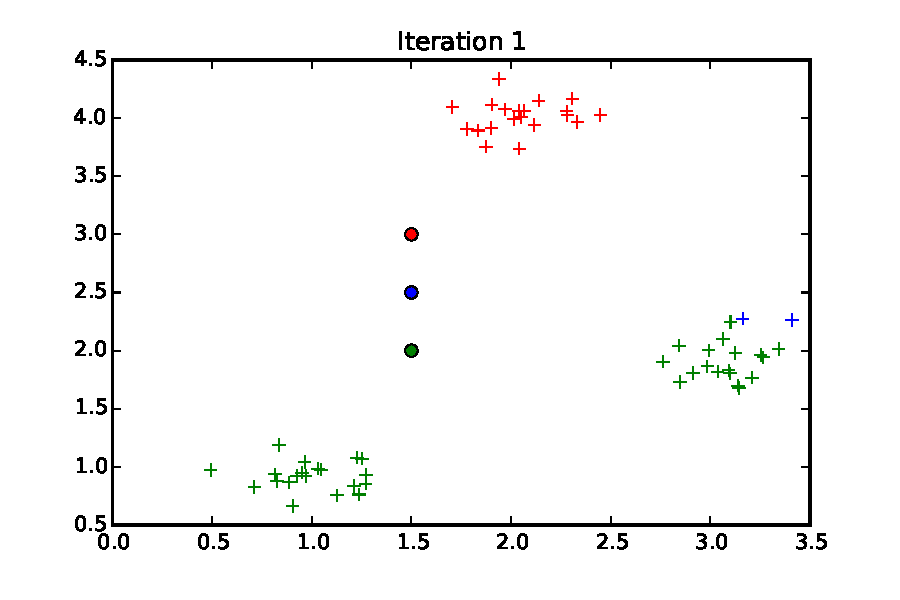
\includegraphics[width=0.7\linewidth]{images/iteration01}
\caption{k-Means: Possible initial centroid positions}
\label{fig:kmeans:iteration01}
\end{figure}

\begin{figure}
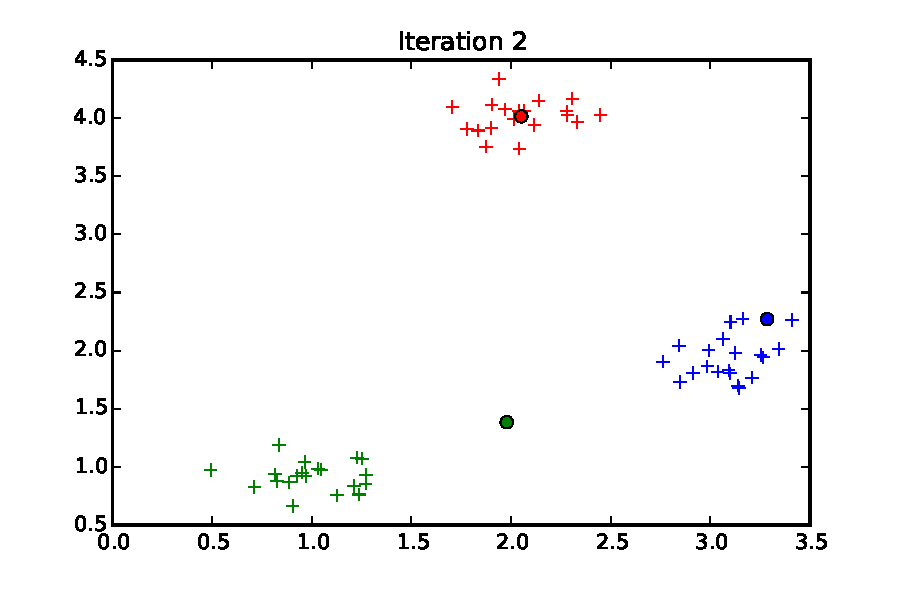
\includegraphics[width=0.7\linewidth]{images/iteration02}
\caption{k-Means: First iteration}
\label{fig:kmeans:iteration02}
\end{figure}

\begin{figure}
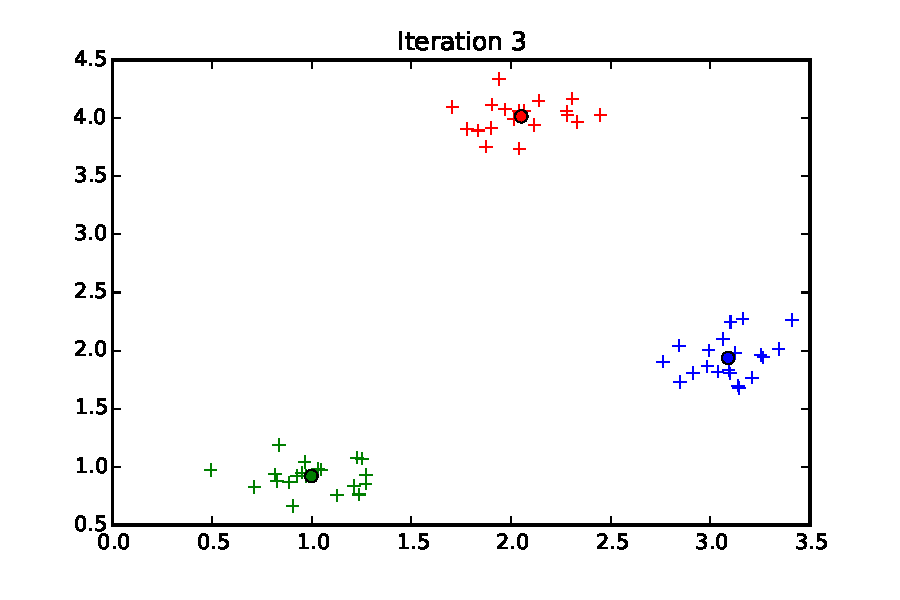
\includegraphics[width=0.7\linewidth]{images/iteration03}
\caption{k-Means: Second iteration}
\label{fig:kmeans:iteration03}
\end{figure}


This means that the k-means algorithm tries to optimize the objective function \ref{eqn:kmeans_objective_function}. As there are only a finite number of possible assignments for the amount of centroids and observations available and each iteration has to result in better solution, the algorithm always ends in a local minimum.

\begin{equation}
J = \sum_{n=1}^{N} \sum_{k=1}^{K} r_{nk} ||x_n - \mu_k||^2
\label{eqn:kmeans_objective_function}
\end{equation}

\[
\text{with } \\
r_{nk} = \begin{cases}
%1 & \text{if } k = \arg \min_j ||x_n - \mu_j||^2 \\
1 & x_n \in S_k \\
0 & \text{otherwise}
\end{cases}
\]

% minimize graph image

The main problem of k-means is his dependency to the initial chosen centroids. The centroids could end up in splitting common data points whilst other, separated points get grouped together if some of the points are more attracted by outliers of multiple points get pulled to the same group of data points as shown in figure \ref{fig:kmeans_bad}.


\begin{figure}[h]
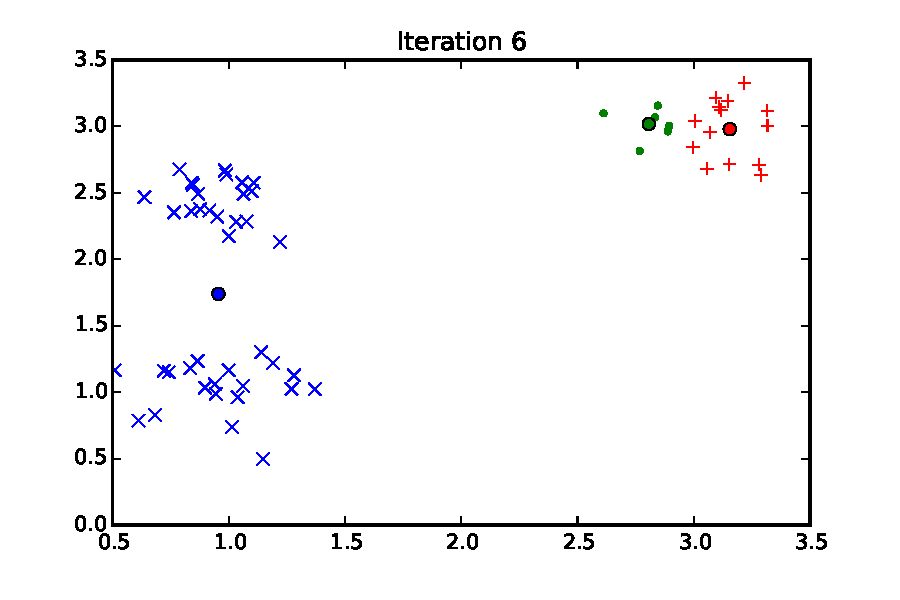
\includegraphics[width=0.7\linewidth]{images/kmeans_bad}
\caption{k-Means: Bad chosen initial center points}
\label{fig:kmeans_bad}
\end{figure}

The most common approach is to perform multiple clusterings with different start positions. Afterwards the most occurred clustering is considered as correct. Another, newer approach is the so called k-means++ by Arthur and Vassilvitskii \cite{Arthur:2007:KAC:1283383.1283494}. This extension to the k-means algorithm tries to distribute the initial centroids over the given data to minimize the probability of bad outcomes. The initial points are set according to the authors by the following steps

\begin{enumerate}
    \item Take uniformly a random data point from the data $X$ and mark it as centroid $c_1$
    \item Choose another centroid $c_i$ with the probability $\frac{D(x)^2}{\sum_{x \in X} D(x)^2}$ where $D(x)$ denotes the shortest distance from the data point $x$ to its closed, already chosen centroid.
    \item Repeat 2. until all $k$ initial centroids are chosen.
\end{enumerate}

Afterwards, the standard k-means algorithm as described above is performed. The authors also showed that with this initialization algorithm, k-means++ approximately can be computed in $O(\log n)$, compared to $O(n^{dk+1} \log n)$ for the standard algorithm.
